\chaptermark{Introduction}
\chapter{Introduction}
\label{ch:introduction}
The Greek philosopher Heraclitus once said that one constant since the beginning of time is change. However, the fear of change is also a constant.  His central claim is summed up in the phrase Panta Rhei ("life is flux"), recognising life's essential, underlying essence as change. Nothing in life is permanent, nor can it be, because the very nature of existence is change. Since times immemorial, humans have liked routine, making us feel in control of our lives. When that fear of change becomes irrational, our ability to control it becomes a phobia, particularly Metathesiophobia. A Metathesiophobe feels they have no control over their lives due to constant change. Metathesiophobes tend to live in the past and are unwilling to progress, often leading to depression, seriously impacting their professional and personal lives. If a society or country rejects the change, there is no growth and no progress. The inability to change, progress, or grow can result in stagnation. Stagnation rejects realising ones full potential. Stagnation is not a healthy flowing river; it is an idle and stale pond. \parencite{Mark2010, Arapahoe2020}

A world that is continuously in flux is a \acrfull{vuca} world. According to \textcite{Bennett2014} the world of \acrshort{vuca} requires a new approach. Disintermediation, globalisation, market upheaval, disruption, and technological advance all combine to produce an effect that is difficult to mitigate,  impossible to predict, and arduous to detect \parencite[p. 885]{OReilly2019}. \textcite{Taleb2008} his definition of a black swan (see later in this chapter) is similar. To deal with the \acrshort{vuca} world, companies invested a great deal of time and money in becoming less \gls{fragile} by being more \gls{agile}, \gls{robust} and \gls{resilient}. However, \textcite{Taleb2012} claims by being more \gls{agile}, \gls{robust}, or \gls{resilient}, the company can only withstand the change but does not gain from it.

\textcite{Taleb2012} defines the opposite state of \gls{fragile}, \gls{antifragile} as an answer to what \textcite{Taleb2008} calls black swan events. These black swan events are also known as X-events \parencite{Casti2013}. \textcite{Taleb2012} states that \gls{resilient}, \gls{robust} (and company) are states that neither breaks nor improves. \textcite{Taleb2012} claims that \gls{antifragile} is the state that gains and improves. \Gls{antifragile} is the true opposite of \gls{fragile}.

In this thesis, I define the \acrfull{ea} success factors for contribution to become \gls{antifragile}. I use the contextual boundary of the public sector as my lens.

\section{The author}
\label{sec:context}
I am working as a Chief Architect for an \acrfull{isv} specialised in delivering software and services to the local governmental agencies in The Netherlands, such as municipalities, the provinces, the local tax offices, and the regional water authorities. 

\section{The structure of this thesis}
\label{sec:structure}
In chapter \ref{ch:introduction}, the context of the research is set, the core concepts of \acrshort{ea} and \glspl{antifragile} are introduced together with the contextual boundary of the public sector. This chapter is closed with the problem statement, the belonging research questions, and the substantiation of the relevance of this research.

In chapter \ref{ch:theoreticalbackground}, the background is given based on literature research. The contextual boundary of the public sector is defined. The concepts of \acrshort{ea}, \gls{antifragile}, and other relevant concepts such as system, organisation, and stressor are researched and defined in detail. 

Chapter \ref{ch:research-methodology} explains the used research methodology and the approach for the research based on the FAIR\footnote{\url{https://www.go-fair.org/fair-principles/}} principles and the research properties of replicability, falsification, independence, and precision as described by \textcite{Recker2013}.

I will elaborate on the fact that the public sector suffers from the digital transformation and the increase in the speed of change in chapter \ref{ch:vucaandpublicsector}. The \acrfull{vuca} world \parencite{Bennett2014} is used as a lens in this chapter.

\section{Introduction of the public sector}
\label{sec:intropublicsector}
According to \textcite{PrivacySense2016} the public sector is comprised of organisations that are owned and operated by the government and exist to provide services for its citizens. Similar to the non profit sector, organisations in the public sector do not seek to generate a profit. Sometimes the public sector will partner with an organisation in the private sector to create a public-private partnership. These hybrid organisations work together to deliver a service or business venture to a community jointly. Through outsourcing, public sector organisations will often engage the private sector to deliver goods and services to their citizens.

I argue that, in the hybrid model, the definition of the public sector is not correct anymore. The part of a private company that is a part of a hybrid collaboration with the public sector should be part of the definition of the public sector.

\begin{figure}[H]
	\centering
	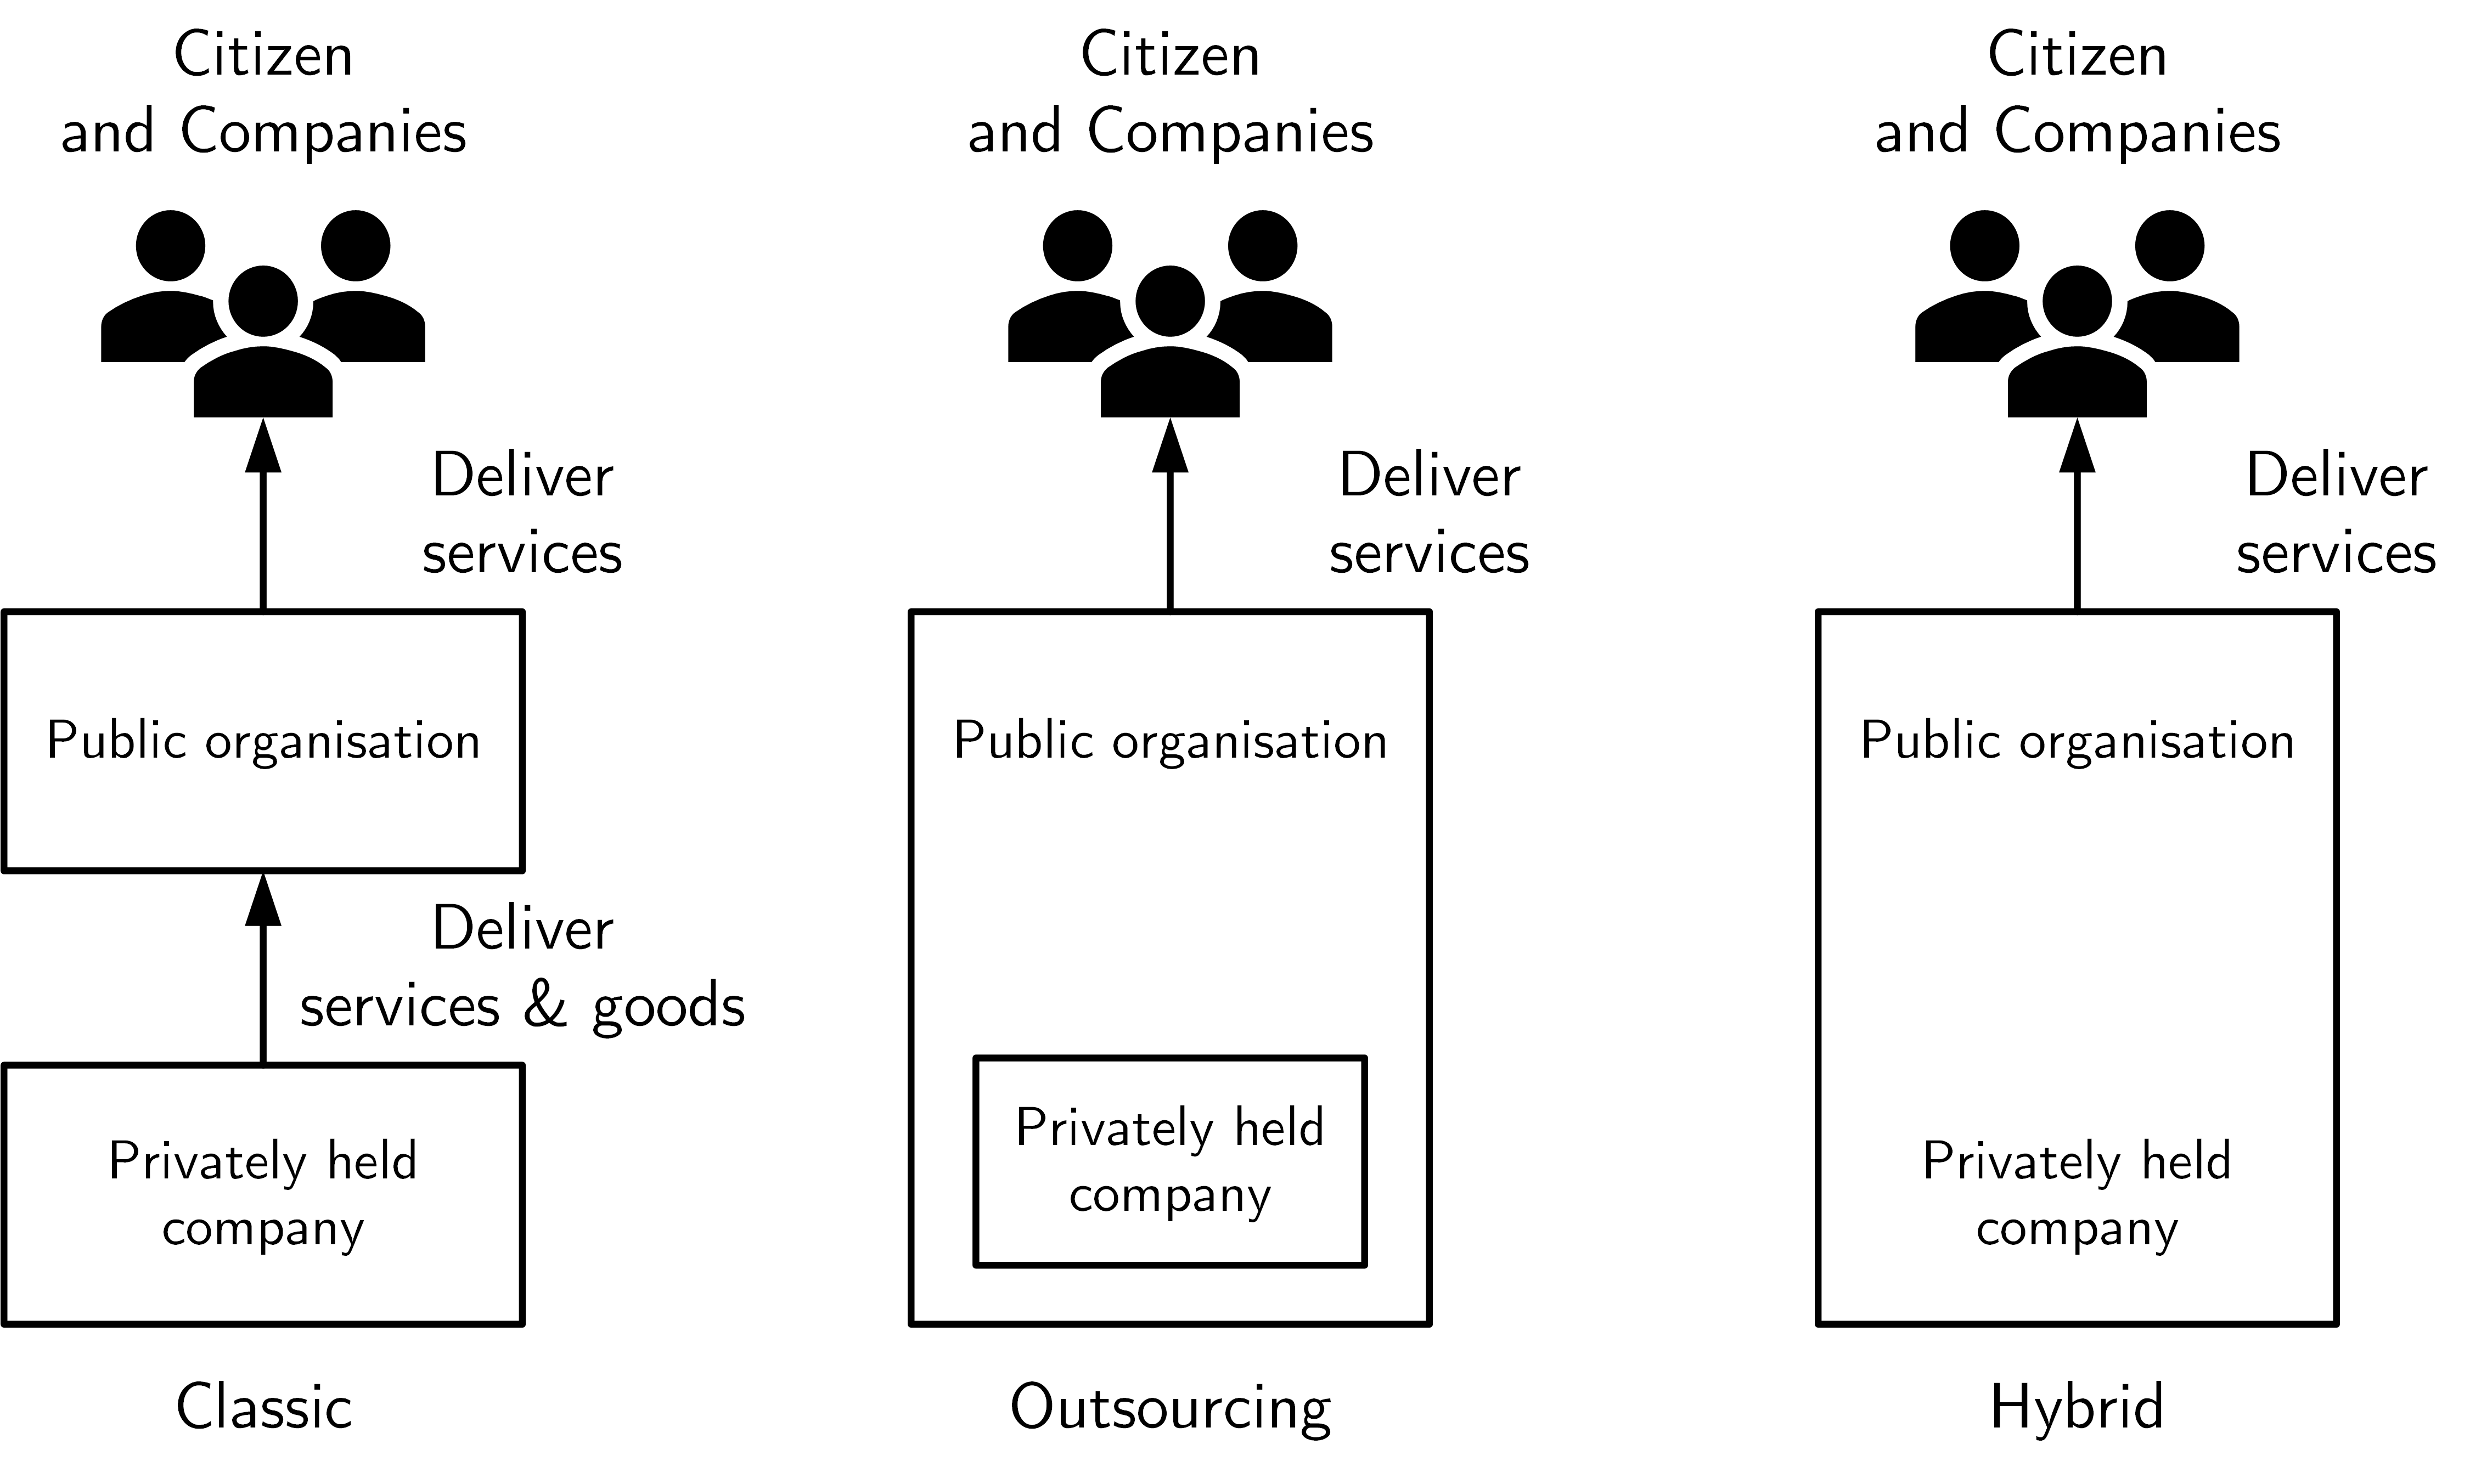
\includegraphics[width=0.7\linewidth]{images/publicsector3modelsofcolaboration}
	\caption[Public sector collaboration models]{Public sector collaboration models}
	\label{fig:publicsector3modelsofcolaboration}
\end{figure}

The public sector is divided into three levels \parencite{PrivacySense2016}:

\begin{itemize}
	\item{\textbf{The national government,} such as the military, the tax authority, and homeland affairs.}
	\item{\textbf{The regional government,} such as the provinces, the police, and water management.}
	\item{\textbf{The local government,} such as the municipalities, the social services, and the local tax offices.}
\end{itemize}

I will focus this research on the public sector level local government (of the Netherlands).

The core values are different in the public sector than that of the private sector. The top five private sector core values are profitability, accountability, expertise, reliability, and effectiveness. The top five public sector core values are accountability, effectiveness, incorruptibility, reliability, and lawfulness. \parencite{Wal2008} Profitability is only a value for the private sector, and it does not exist as a value for the public sector.  The public sector demands or even initiates changes without noticing the needed investments to execute these changes by the private sector.

\begin{remark}
	For hybrid collaborations and partnerships add the reference to iBestuur congress of 2021 about the necessity for the public and private sector to work closely together. Public Sector sees this as necessary to speed up innovation. The reference is expected first week of October 2021.
\end{remark}

\begin{remark}
	The analysis of the 3 types of collaboration should go to the theoretical background. Is necessary to state that the public sector includes privately held companies in some way. Possible even a System-of-Systems.
\end{remark}

\begin{remark}
	Local government is influenced by national government because of policies and regulations.
\end{remark}

\section{Introduction of the concept Enterprise Architecture}
\label{introea}
\acrfull{ea} is a discipline for proactively and holistically leading enterprise responses to disruptive forces by identifying and analysing the execution of change toward desired business vision and outcomes. \acrshort{ea} delivers value by presenting business and IT leaders with signature-ready recommendations for adjusting policies and projects to achieve targeted business outcomes that capitalise on relevant business disruptions \parencite{Gartner}.

\textcite{White2018} states that the organisation’s business requirements guide \acrshort{ea} — it helps layout how information, business and technology flow together. \acrshort{ea} has become a priority for businesses trying to keep up with new technologies such as the cloud, \acrfull{iot}, machine learning and other emerging trends that will prompt digital transformation.

IEEE Definition


\section{Introduction of the concept of antifragility}
\label{sec:introantifragility}
\textcite{Taleb2008} describes a black swan as an event that 1) is so rare that even the possibility that it might occur is unknown, 2) has a catastrophic impact when it does occur, and 3) is explained in hindsight as if it were actually predictable. For extremely rare events, \citeauthor{Taleb2008} argues that the standard tools of probability and prediction, such as the normal distribution, do not apply since they depend on large population and past sample sizes that are never available for rare events by definition. Extrapolating, using statistics based on observations of past events is not helpful for predicting black swans, and might even make us more vulnerable to them. In his book \Gls{antifragile}, \textcite{Taleb2012} states that the way to survive a black swan event is to be \gls{antifragile}.\par
Most people answer that the opposite of \gls{fragile} is \gls{robust}, \gls{resilient}, solid, or something of the sort. However, the \gls{resilient}, \gls{robust} (and company) are items that neither break nor improve, so you would not need to write anything on them — have you ever seen a package with \gls{robust} in thick green letters stamped on it? Logically, the exact opposite of a \gls{fragile} parcel would be a package on which one has written, please mishandle or please handle carelessly. Its contents would not just be unbreakable but would benefit from shocks and a wide array of trauma \parencite{Taleb2012}.

\begin{figure}[h!]
	\centering
	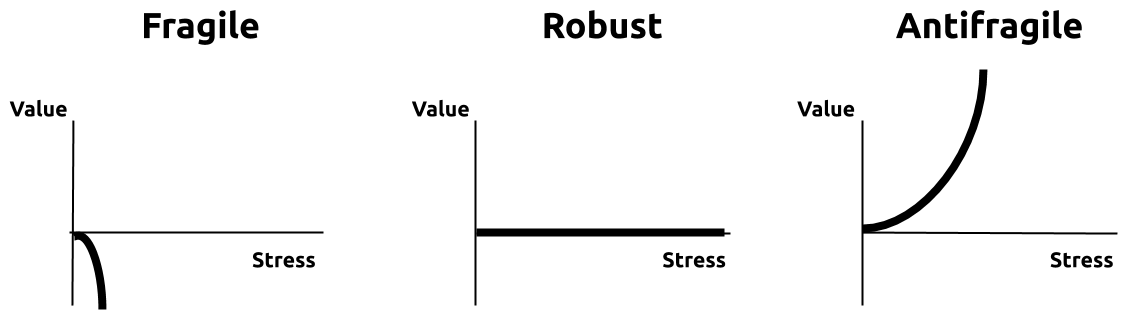
\includegraphics[width=0.7\linewidth]{images/eaal-triad}
	\caption[EAAL Triad]{\acrshort{eaal} Triad \parencite{Botjes2020}}
	\label{fig:eaal-triad}
\end{figure}

\section{Problem statement}
\label{sec:problemstatement}
The concept of \gls{antifragility} implies that organisations could benefit and strengthen from crises, volatility, errors and uncertainty and could also lead to opportunities for innovation \parencite{Kastner2017}. Enterprise Architecture is a discipline that helps organisations to reach their goals. As stated by \textcite{Gartner} \acrshort{ea} is a discipline for proactively and holistically leading enterprise responses to disruptive forces by identifying and analysing the execution of change toward desired business vision and outcomes. One would expect that an organisation uses the discipline of \acrshort{ea} to get more towards the state of \gls{antifragility}. Research has been conducted on aspect architectures such as the application and information architectures but not on \acrshort{ea}. The problem is that the Body of Knowledge contains no direct knowledge on how to achieve \gls{antifragility} with the use of \acrshort{ea}. 

\section{The research subject}
\label{sec:researchsubject}
\acrshort{ea} facilitates an organisation in assessing the impact of change and making recommendations for target states that support business objectives. \acrshort{ea} guides an organisation in changing. \acrshort{ea} can help organisations in changing towards the state of \gls{antifragility}. However, what are the success factors of \acrshort{ea} that contribute in accomplishing \gls{antifragility}? This is summarised in a conceptual research model.
\begin{figure}[H]
	\centering
	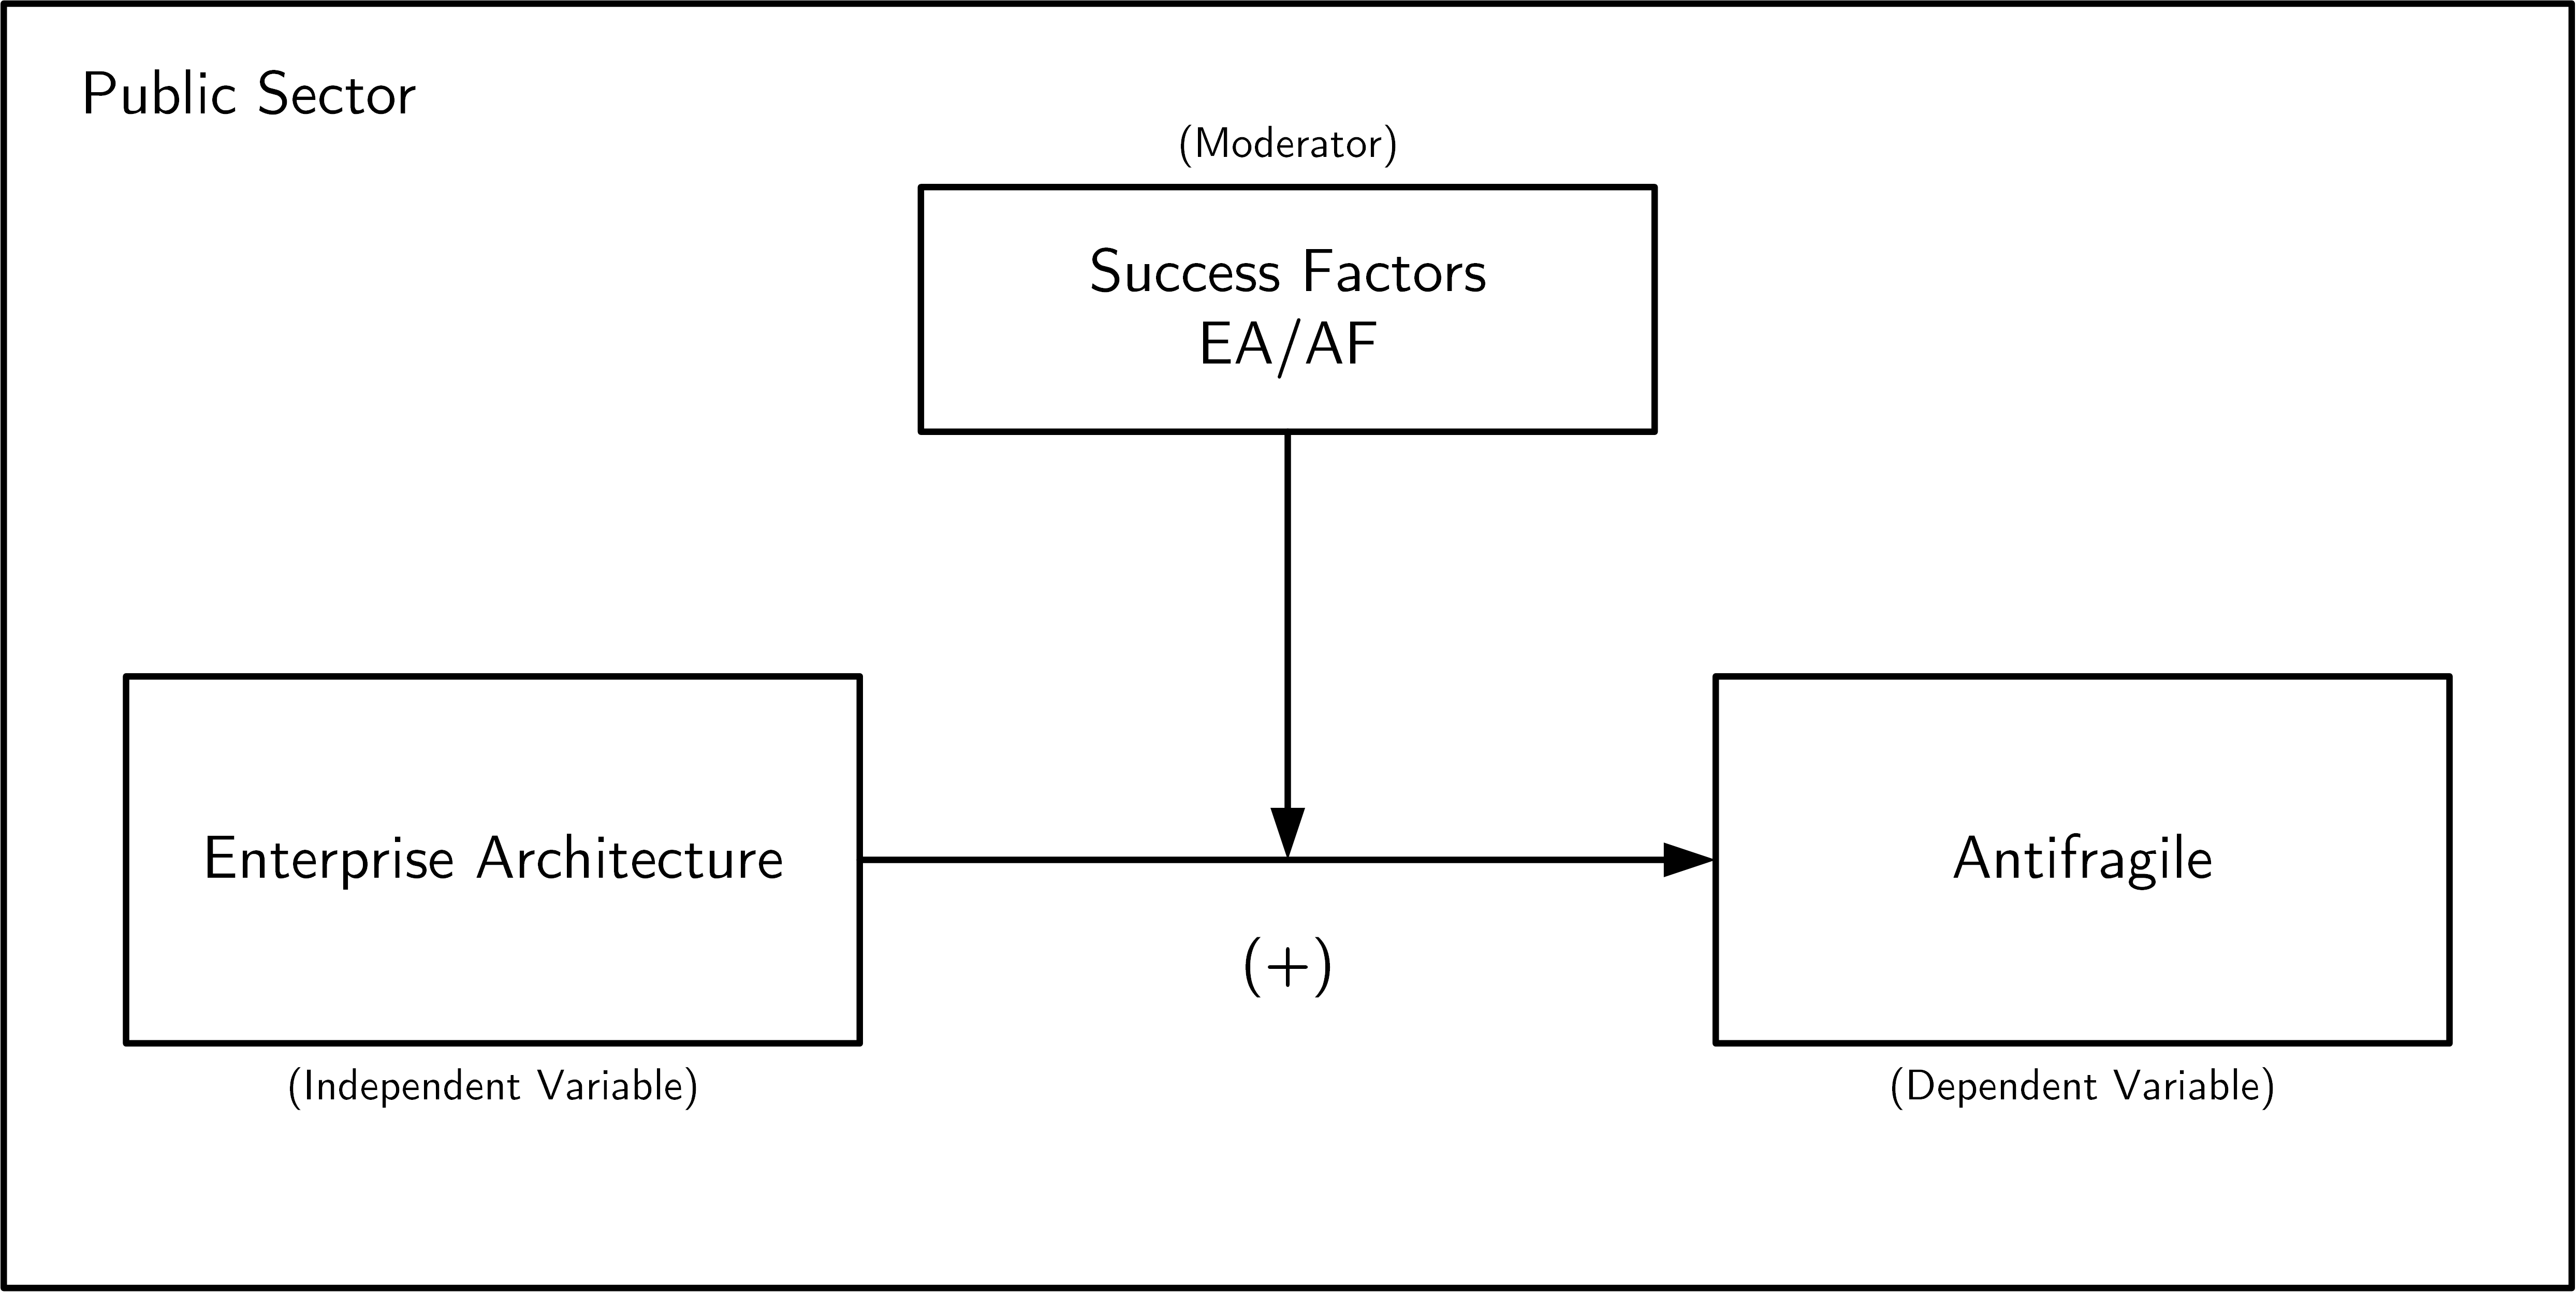
\includegraphics[width=0.8\linewidth]{images/conceptualmodel}
	\caption[Conceptual Research Model]{Conceptual Research Model}
	\label{fig:conceptualmodel}
\end{figure}
The hypothesis of the conceptual research model is that, in the context of the public sector, \acrlong{ea} Success Factors have a positive influence in the contribution of \acrlong{ea} in achieving antifragility. From this conceptual research model the research question can be stated as:\bigskip

\noindent \emph{''What are the success factors of \acrlong{ea} for \gls{antifragility} in the public sector?''}\bigskip

\noindent To correctly answer this research question the following sub-questions need to be answered:

\begin{enumerate}
	\item{What is literature saying about the public sector?}
	\item{What is literature saying about \acrlong{ea}?}
	\item{What is literature saying about the success factors of Enterprise Architecture?}
	\item{What does literature say about antifragile?}
%	\item{How can the success factors of \acrlong{ea} contribute to becoming antifragile?}
\end{enumerate}
\section{Research relevance}
\label{sec:researchrelevance}
%\begin{wrapfigure}{R}{0.3\textwidth}
%	\centering
%	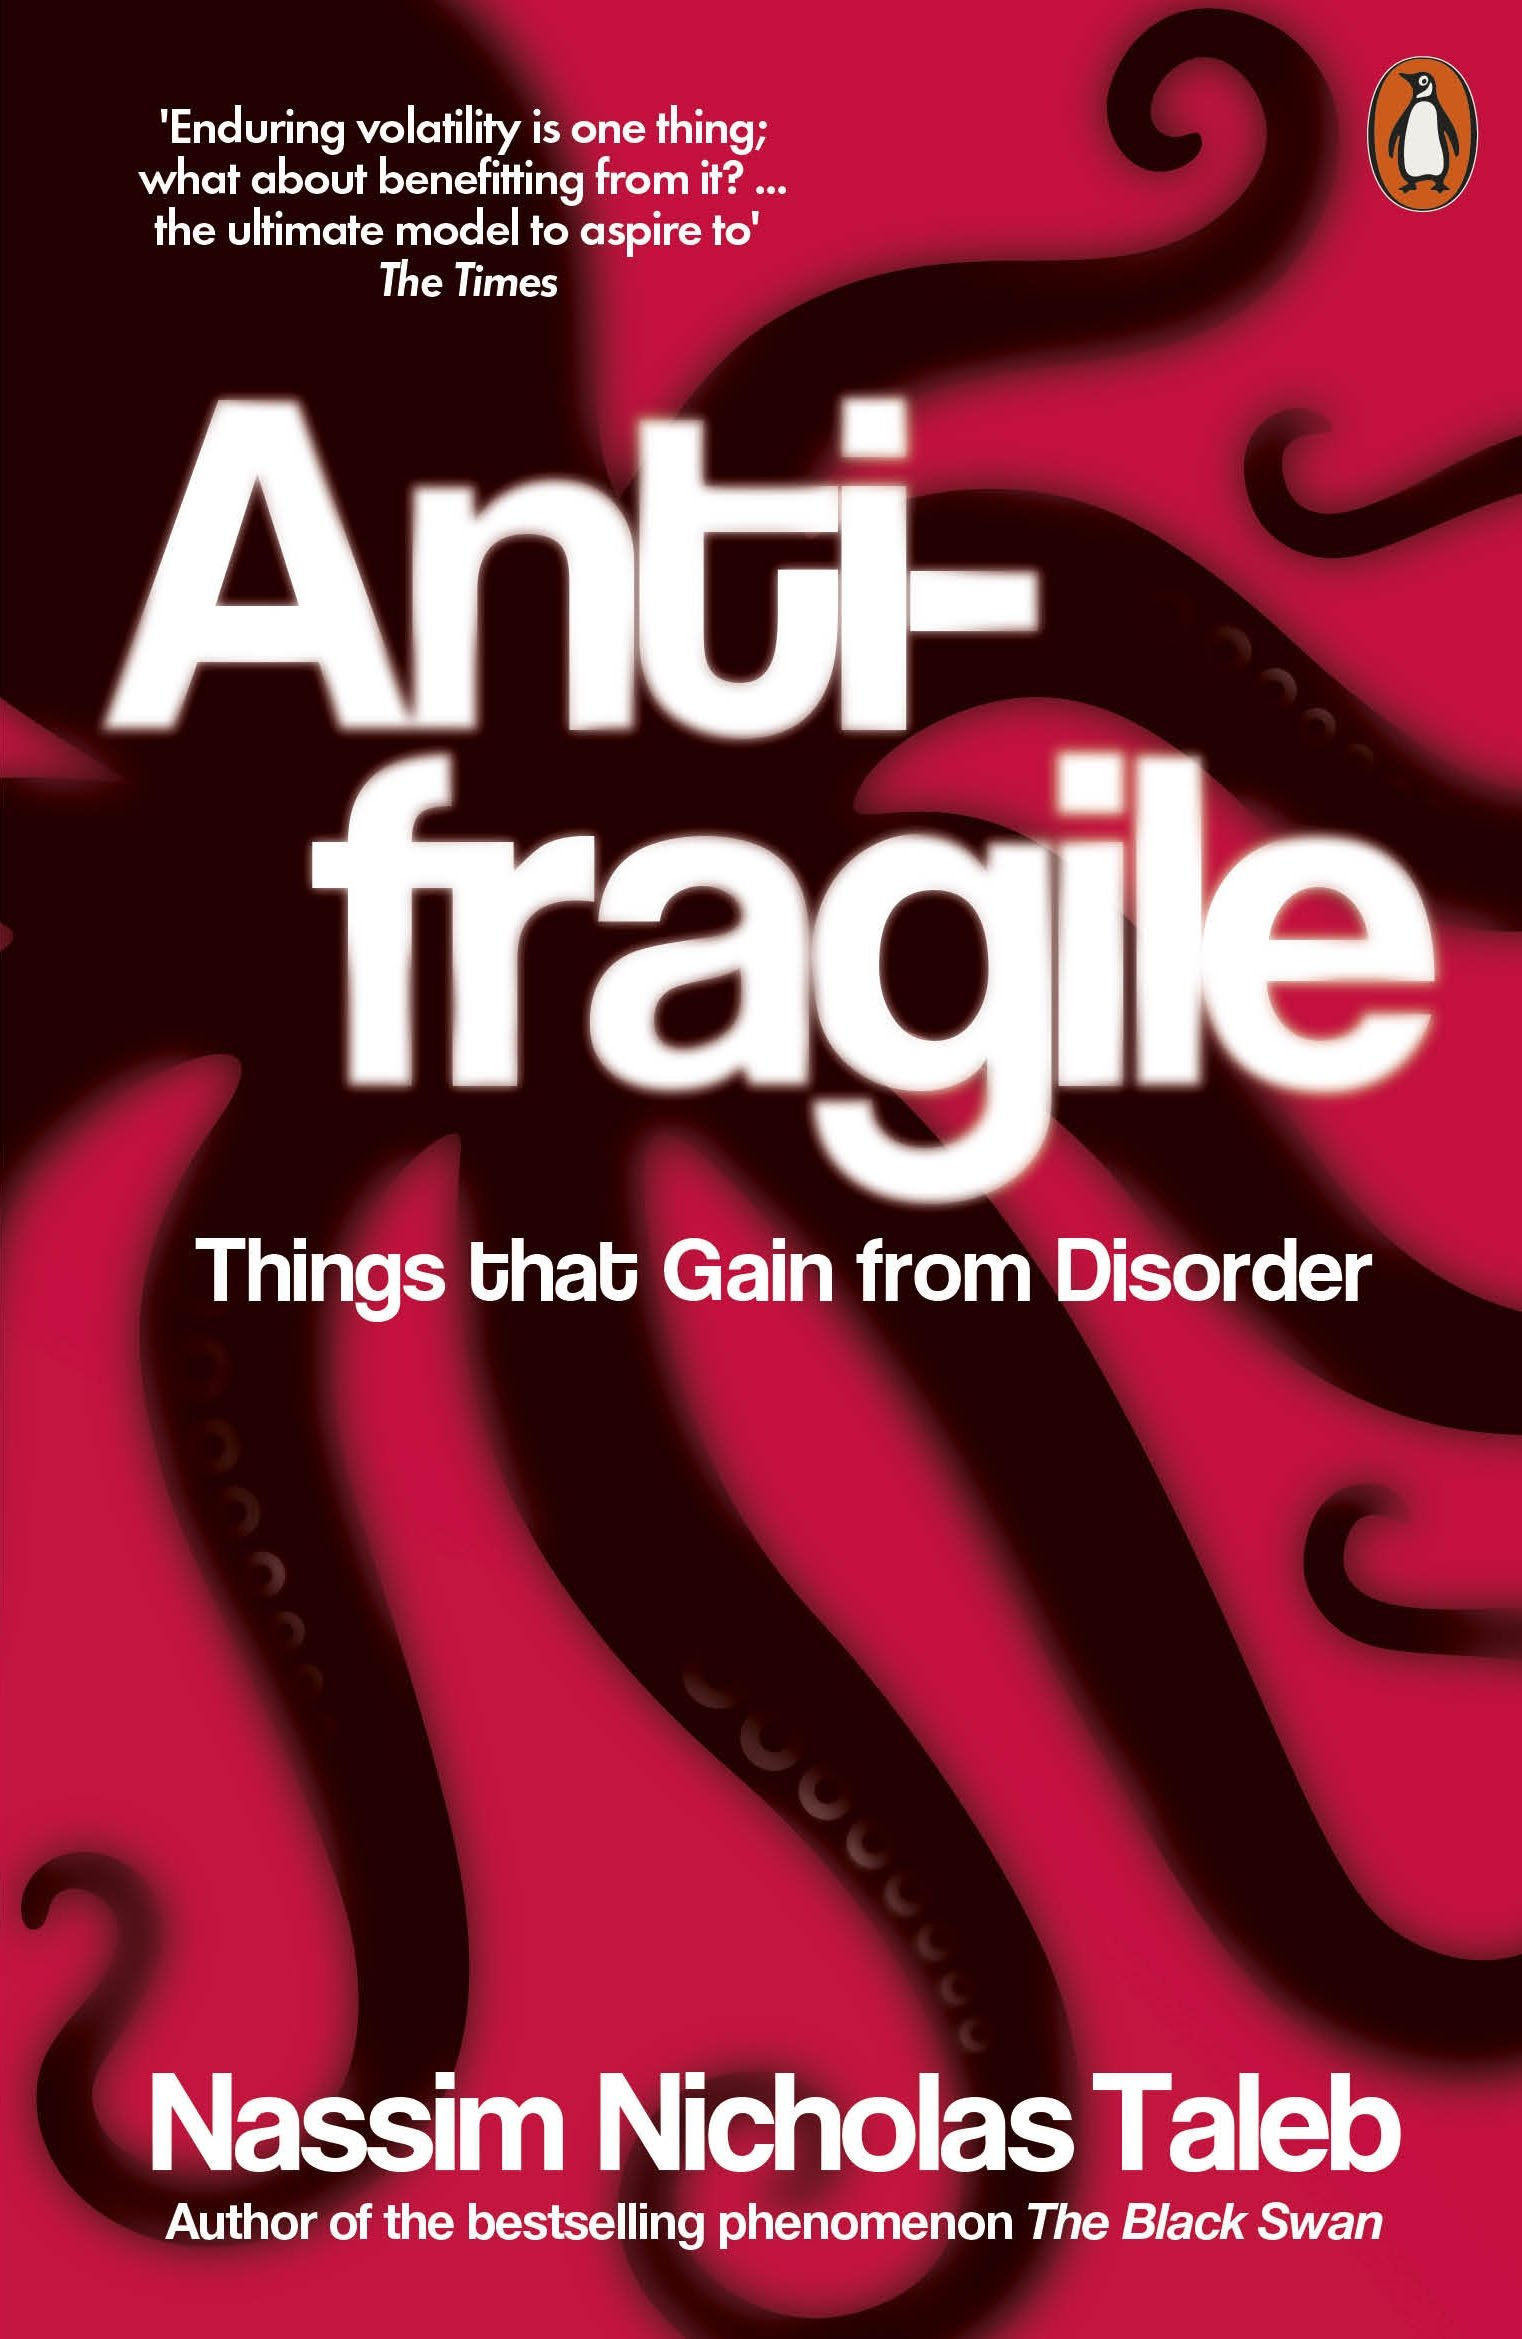
\includegraphics[width=0.28\textwidth]{images/antifragilebookcover.jpg}
%	\caption{Antifragile: Things that gain from disorder}
%\end{wrapfigure}
\acrfull{ea} has contributed to being more \gls{robust}, \gls{resilient}, and \gls{agile}. Using \acrshort{ea} in pursuing \gls{antifragility} will add value to companies by accelerating and growing when there is a stressor or black swan event. The \gls{antifragile} theory is young.  \citeauthor{Taleb2012} published the theory in his book ''\Gls{antifragile}: Things that gain from disorder.'' in \citeyear{Taleb2012}.  Studies conducted on \acrshort{ea} with the concept of \gls{antifragile} are almost non-existence. The conducted studies are primarily about making IT Systems \gls{antifragile}. \textcite{Botjes2020,Kastner2017} are exceptions and have researched how to apply \gls{antifragile} in an organisational context. Nevertheless, both concluded that there is more research needed. The former used the lens of Enterprise Engineering, which is closely related to \acrshort{ea}, together with resilience, while the latter used mostly reslience as its lens. There is still no answer to how \acrshort{ea} can contribute to becoming \gls{antifragile}. Organisations use the practice of \acrshort{ea} to guide them to achieve their goals. Giving more insights on this subject will contribute to the Body of Knowledge and help others getting closer to \gls{antifragility} by using \acrshort{ea}.

Because of the digital transformation, the pace of change is increasing rapidly. The increase in pace is not only seen in the private sector but also the public sector. The public sector has another change dimension; elections result in changed regulations and governmental policies. These changes are a result of a new political agenda. In the past, the chosen direction was stable for at least the period until the new elections. With the digital transformation the changes are also taking place in between elections with an increase of pace. Earlier chosen directions often result in the need for a new approach and even new directions. Earlier made investments can be made obsolete because of the new directions that follow out of those policies. The products and services that are delivered are, over time, unpredictable in use and functionality. To overcome this problem, most companies invest a great deal of time and money in being less fragile when the market changes or disruptions occur. This investment is to withstand changes by being more agile, robust, and resilient. By being more agile, robust, or resilient, the company can only withstand the change or the disruption but does not gain from it. See for more information chapter \ref{ch:vucaandpublicsector}. Governmental agencies and suppliers in the public sector are searching for methods of dealing with this increased pace and the disruptions that occur. The relevance of this research is not only about the addition to the Body of Knowledge but also to share the outcome with the public sector.

\begin{remark}
	These statements will be verified by interviews and the outcome of these interviews are part of \ref{ch:vucaandpublicsector}.
	This section needs some work! The context of the \gls{ps} is not part of the first part of the relevance... (work in progress)
\end{remark}

\Gls{ps}